\documentclass[11pt]{article}
\usepackage[utf8]{inputenc}
\usepackage[english]{babel}
\usepackage{bilal2vec}

\title{SE 380 — HW 5}
\author{Bilal Khan\\
\href{mailto:bilal2vec@gmail.com}{bilal2vec@gmail.com}}
\date{\today}

\begin{document}

\maketitle

\tableofcontents

\section{1}

Design a lead-lag compensator $C(s)$ to control the system

\[ G(s) = \dfrac{1}{(1 + s)^3} \]


such that $L(s) = C(s)G(s)$ has steady-state gain greater than 100, crossover frequency greater than 5, and phase margin greater than $60^\circ$.

We will design a controller with two parts $C_1(s) = \dfrac{1}{(1 + s/p_1)(1 + s/p_2)^3}$ where $p_1, p_2$ are pole locations. This part is used to set the crossover frequency and make the controller realizable by increasing the degree of the denominator. We arbitrarily choose $\omega_c = 10$ as our crossover frequency and place poles one decade before and one decade after it. Note that the phase margin should be $90^\circ$ as the pole one decade before the crossover frequency will contribute a phase of $-90^\circ$ to the bode plot. We place three poles one decade after the crossover frequency to ensure that our final controller will be realizable.

\[ C_1(s) = \dfrac{1}{(1 + (s / 1)) (1 + (s / 100)^3)} \]

To satisfy the steady state gain requirement, we need $F(0) \geq 100$ and so we choose a steady state gain of $101$. We use a phase-lag controller to improve static performance withouth losing stability: $C_2(s) = \mu \frac{1 + T s}{1 + \alpha T s}$. We choose the default value of $\alpha = 10$ and $T = 10 / \omega_c$ to limit the phase margin decrease at the crossover frequency to $\approx 6\%$, which gives us more than enough phase margin to satisfy the requirement. We choose $\mu = 101$ since we know that phase-lag controllers increase the steady state gain at low frequencies (and by extension the steady-state gain) by a factor of $\mu$.

\[ C_2(s) = 101 \dfrac{1 + s}{1 + 10s} \]

We then combine the two controllers and cancel out the $G(s)$ to get our final controller. Note that the controller is proper.

\[ C(s) = C_1(s) C_2(s) / G(s) = 101 \dfrac{1}{(1 + (s / 1)) (1 + (s / 100)^3)} \dfrac{1 + s}{1 + 10s} \dfrac{(1 + s)^3}{1} \]

In code:

\begin{minted}{python}
import math
import numpy as np
import control as ct
import matplotlib.pyplot as plt

s = ct.tf('s')
G = 1 / (1 + s)**3

plt.figure()
ct.bode_plot(G, margins=True)
plt.show()

plt.figure()
t, y = ct.step_response(G)
plt.plot(t, y)
plt.show()

omega_c = 10

pole_1 = omega_c / 10
pole_2 = omega_c / 0.1
C_1 = 1 / ((1 + (s / pole_1)) * (1 + (s / pole_2)) ** 3)

alpha_2 = 10
mu_2 = 101
T_2 = 10 / omega_c
C_2 = mu_2 * (1 + T_2 * s) / (1 + alpha_2 * T_2 * s)

C = C_1 * C_2 * (1 / G)

plt.figure()
ct.bode_plot(C * G, margins=True)
plt.show()

plt.figure()
t, y = ct.step_response(C * G)
plt.plot(t, y)
plt.show()
\end{minted}

$G(s)$ bode plot

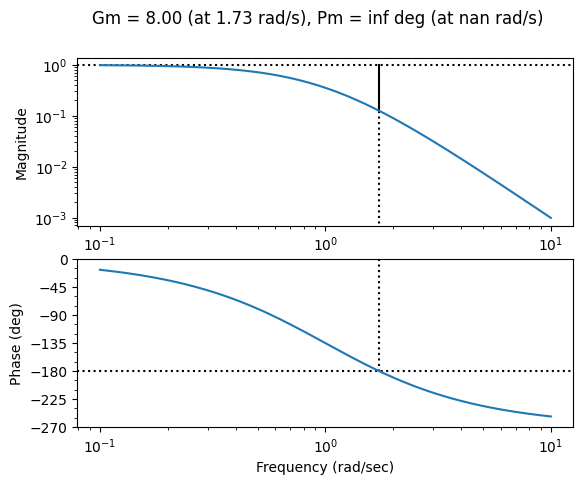
\includegraphics[width=300pt]{a5_1.png}

$G(s)$ step response

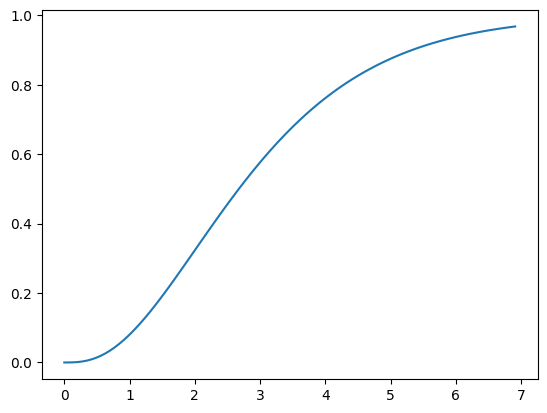
\includegraphics[width=300pt]{a5_2.png}

$C(s)$ bode plot

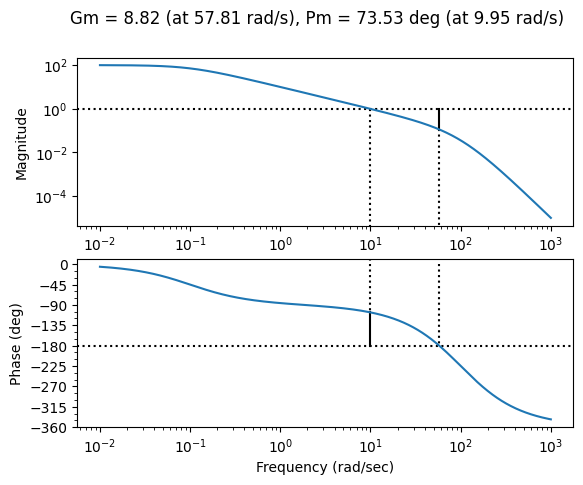
\includegraphics[width=300pt]{a5_3.png}

$C(s)$ step response

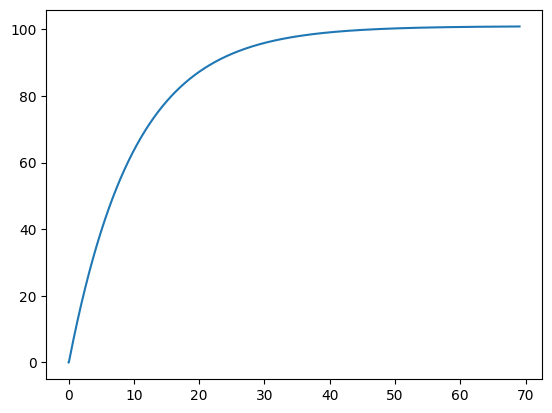
\includegraphics[width=300pt]{a5_4.png}

\section{2}

Design a proportional controller for the system $G(s) = \frac{100(s + 1)}{(s - 1)(s^2 + 5s + 10)}$ such that the closed-loop system is stble and the damping of the complex-conjugate poles is greater than $0.45$. Note from the textbook that the phase margin of a second order system is approximately equal to 100 times the damping of the poles as long as the phase margin in between 0 and 60 degrees. A proportional controller is of the form $C(s) = k_p$. Through trial and error we find that $k_p = 0.2$ satisfies the phase margin requirements.

In code:

\begin{minted}{python}
import math
import numpy as np
import control as ct
import matplotlib.pyplot as plt

s = ct.tf('s')
G = (100 * (s + 1)) / ((s - 1) * (s**2 + 5 * s + 10))

plt.figure()
ct.bode_plot(G, margins=True)
plt.show()

plt.figure()
t, y = ct.step_response(G / (1 + G))
plt.plot(t, y)
plt.show()

s = ct.tf('s')
G = (100 * (s + 1)) / ((s - 1) * (s**2 + 5 * s + 10))

plt.figure()
ct.bode_plot(0.2 * G, margins=True)
plt.show()

plt.figure()
t, y = ct.step_response(G / (1 + G))
plt.plot(t, y)
plt.show()
\end{minted}

$G(s)$ bode plot

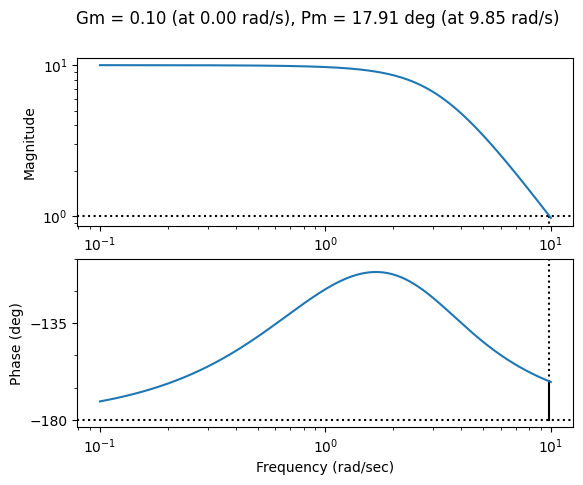
\includegraphics[width=300pt]{a5_5.png}

$G(s)$ step response

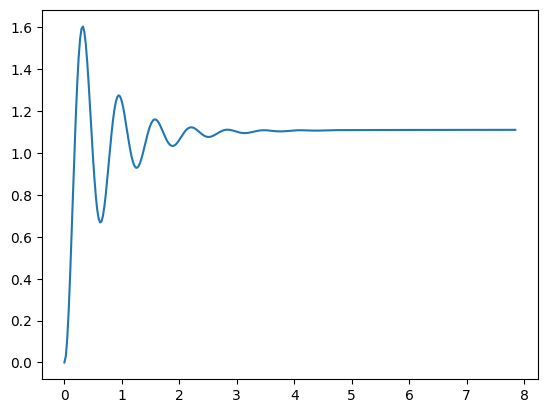
\includegraphics[width=300pt]{a5_6.png}

$C(s)$ bode plot

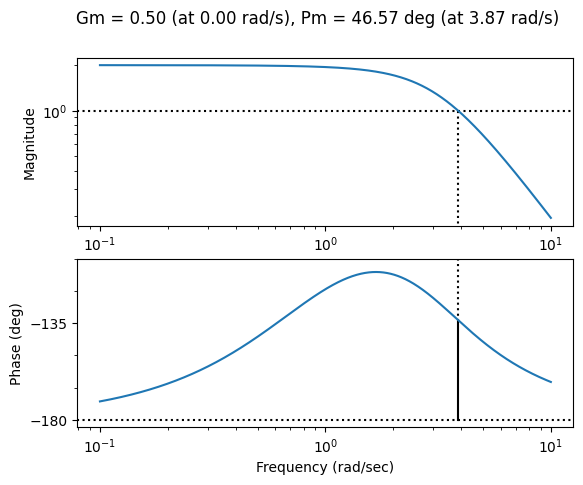
\includegraphics[width=300pt]{a5_7.png}

$C(s)$ step response

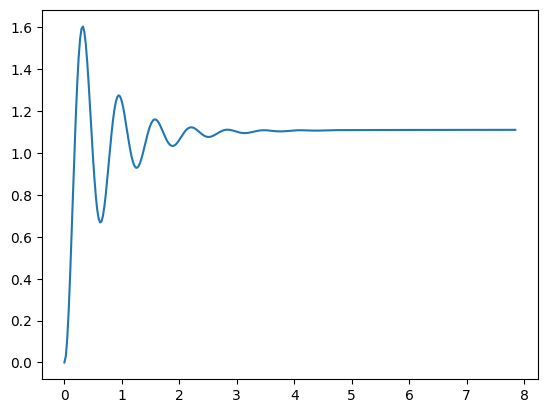
\includegraphics[width=300pt]{a5_8.png}


\end{document}
